%Dokumentklasse
\documentclass[a4paper,12pt]{scrreprt}
\usepackage[left= 2.5cm,right = 2cm, bottom = 4 cm]{geometry}
%\usepackage[onehalfspacing]{setspace}
% ============= Packages =============

% Dokumentinformationen
\usepackage[
	pdftitle={Titel der Abschlussarbeit},
	pdfsubject={},
	pdfauthor={Euer Name},
	pdfkeywords={}
	pdftex=true, 
	colorlinks=true,
 	breaklinks=true,
	citecolor=black,
	linkcolor=black,	
	menucolor=black,	
	urlcolor=black
]{hyperref}


% Standard Packages
\usepackage[utf8]{inputenc}
\usepackage[ngerman]{babel}
\usepackage[T1]{fontenc}
\usepackage{graphicx}
\graphicspath{{img/}}
\usepackage{fancyhdr}
\usepackage{lmodern}
\usepackage{color}
\usepackage{transparent}

% zusätzliche Schriftzeichen der American Mathematical Society
\usepackage{amsfonts}
\usepackage{amsmath}

% nicht einrücken nach Absatz
\setlength{\parindent}{0pt}


% ============= Kopf- und Fußzeile =============
\pagestyle{fancy}
%
\lhead{}
\chead{}
\rhead{\slshape \leftmark}
%%
\lfoot{}
\cfoot{}
\rfoot{\thepage}
%%
\renewcommand{\headrulewidth}{0.4pt}
\renewcommand{\footrulewidth}{0pt}

% ============= Package Einstellungen & Sonstiges ============= 

%Besondere Trennungen
\hyphenation{De-zi-mal-tren-nung St-rei-fen-licht-scan-nern}

%römische Aufzählungen mit \RM{Zahl}
\newcommand{\RM}[1]{\MakeUppercase{\romannumeral #1}}


% ============= Dokumentbeginn =============

\begin{document}

\pagestyle{empty}
\begin{center}
\begin{tabular}{p{\textwidth}}


\begin{center}

\includegraphics[scale=0.2]{img/logos.jpg}
\end{center}


\\

\begin{center}
\LARGE{\textsc{
Ein super toller Titel \\
}}
\end{center}

\\


\begin{center}
\large{Fakultät für Muster und Beispiele \\
der Hochschule Musterhausen \\}
\end{center}

\\

\begin{center}
\textbf{\Large{Abschlussarbeit}}
\end{center}



\begin{center}
vorgelegt von
\end{center}

\begin{center}
\large{\textbf{Max Mustermann}} \\
\small{geboren am 01.01.1900 in Musterhausen}
\end{center}

\begin{center}
\large{im Dezember 2014}
\end{center}

\\

\\

\begin{center}
\begin{tabular}{lll}
\textbf{Erstprüfer:} & & Prof. Dr. med. Dr.-Ing. M. Mustermann\\
\textbf{Zweitprüfer:} & &Prof. Dr.-Ing. F. Musterfrau\\
\end{tabular}
\end{center}

\end{tabular}
\end{center}

% \part im Inhaltsverzeichnis nicht nummerieren
\makeatletter
\let\partbackup\l@part
\renewcommand*\l@part[2]{\partbackup{#1}{}}

%Seitennummerierung neu beginnen, Zahlen [arabic], röm.Zahlen [roman,Roman], Buchstaben [alph,Alph]
\pagenumbering{Roman}

\newpage
\addsec{Eidesstattliche Erklärung}
\label{erklaerung}

Hiermit versichere ich, die vorliegende Studienarbeit selbstständig und nur unter Verwendung der von mir angegebenen Quellen und Hilfsmittel verfasst zu haben. Sowohl inhaltlich als auch wörtlich entnommene Inhalte wurden als solche kenntlich gemacht. Die Arbeit hat in dieser oder vergleichbarer Form noch keinem anderem Prüfungsgremium vorgelegen. \\
\\[1.5cm]
Datum:	\hrulefill\enspace Unterschrift: \hrulefill
\\[3.5cm]
 



\addsec{Zusammenfassung / Abstract}
\label{sec:zusammenfassung}
Docker ist eine Software die es ermöglicht Anwendungen zusammen mit ihren Abhängigkeiten in einen isolierten Container zu verpacken.
Diese Arbeit hat es sich zum Ziel gemacht mögliche Anwendungsfälle für die Software Docker aufzuzeigen und diese zu beschreiben.
Zu beginn werden dazu kurz die gängigen Architekturvarianten des Cloud Computing vorgestellt.
Auf dieser Basis werden dann die möglichen Anwendungsbereiche von Docker innerhalb dieser Architekturen vorgestellt und aufgezeigt, dass Docker auch außerhalb des Cloud Computing sinnvoll zur Anwendung gebracht werden kann.
Diese Arbeit geht davon aus, dass dem Leser Docker bereits ein Begriff ist und geht daher nur kurz auf 
die Eigenschaften von Docker selbst ein. Die Betrachtung der Architektur von Docker selbst ist nicht Teil dieser Arbeit.



\newpage
\pagestyle{fancy}
%Inhaltsverzeichnis
\tableofcontents

\newpage
%Seitennummerierung neu beginnen, Zahlen [arabic], röm.Zahlen [roman,Roman], Buchstaben [alph,Alph]
\pagenumbering{arabic}
% pagestyle für gesamtes Dokument aktivieren
\pagestyle{fancy}

\newpage
\chapter{Einleitung}
\label{sec:einleitung}

Cloud Computing gehört derzeit immer noch zu einem der wichtigsten Schlagwörter für Betreiber von IT-Infrastrukturen.
\glqq Eine breit akzeptierte Definition des Begriffs Cloud Computing gibt es bis heute nicht. Allerdings können die grundlegenden Eigenschaften wie folgt zusammengefasst werden: Cloud Computing nutzt Virtualisierung und das Internet zur dynamischen Bereitstellung von IT-Ressourcen. Dabei kann es sich um IT-Infrastrukturen, Plattformen oder Anwendungen aller Art handeln.\grqq \cite[S. 28]{meinel_virtualisierung_2011} Cloudcomputing bezieht sich also sowohl auf Anwendungen, welche als Dienste über das Internet angeboten werden, als auch auf die Hard- und Software, die in Rechenzentren zu deren Bereitstellung benötigt werden.

Virtualisierung und Cloud Computing sind zweit sehr stark miteinander vernetzte Begriffe.
Dabei ist Virtualisierung kein neues Konzept. Bereits in den frühen 60er Jahren entwickelte IBM mit dem Großrechnersystem 360 eine Plattform die aus heutiger Sicht als Vorläufer aller virtuellen Systeme gilt. \cite{frank_balmes_grin_2008}

Heute ermöglicht uns Virtualisierung auf \glqq allen Ebenen von der Entwicklung bis zum Betrieb von Ressourcen, die Vereinheitlichung von Umgebungen und erhöhte Sicherheit durch Isolation. Dies spart Zeit bei der Entwicklung, reduziert Kosten beim Betrieb von Servern und verringert das Fehlerpotential.\grqq \cite[S. 1]{schroder_container-virtualisierung_2014}
Neben der vollwertigen \grq Virtualisierung in Software\grq\ und der \grq Hardware-Virtualisierung\grq\ hat sich noch das Konzept der \grq Virtualisierung mittels Container\grq\ herausgebildet.
\glqq Hier wird eine komplette Betriebssystemumgebung innerhalb eines abgeschlossenen Containers zur Verfügung gestellt. Charakteristisch für diese Virtualisierungsform ist, dass nur ein Kernel des Betriebssystems läuft, der die jeweiligen Container verwaltet und eine saubere Trennung sicherstellt.\grqq \cite{plotner_linux_2012}
Seit der Kernelversion 2.6.29 \cite{fischer_linux_2014} bietet Linux eine Umsetzung dieser Virtualisierungsform bereits als festen Bestandteil des Betriebssystems.
Das Problem mit diesen als LXC bekannten Containern ist jedoch ihr sehr unhandliches Interface.
Das Open Source Projekt Docker der Firma \grq dotCloud\grq\ hat sich diesem Problem angenommen und eine benutzerfreundliche Abstraktionsschicht für die Verwendung von LXC Containern entwickelt. Das Projekt steckt zwar immer noch in den Kinderschuhen, erfreut sich aber schnell wachsender Beliebtheit, wie der Trend der Suchanfragen nach dem Begriff \grq Docker\grq\ zeigt. (siehe Abb \ref{fig:google_trends}) 

\begin{figure}[htb]
  \centering  
  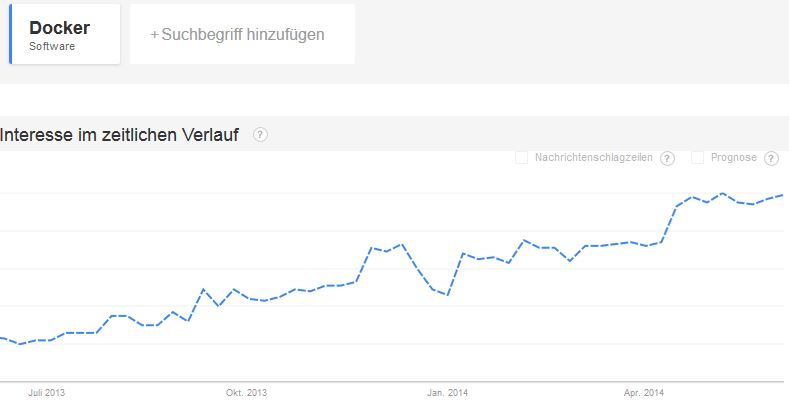
\includegraphics[scale=0.7]{img/docker_trend.JPG}\\
  \footnotesize\sffamily\textbf{Quelle:} \cite{google_trends_google_2014}
  \caption{Trend der Suchanfragen nach dem Begriff \grq Docker\grq\ im Bereich von 07.06.2013 - 07.06.2014 }
  \label{fig:google_trends}
\end{figure}

Schon innerhalb der ersten acht Monaten seit dem Start des Projekts wuchs die Zahl der beitragenden Personen auf über zweihundert an. 
Heute ist Docker bereits in namenhaften Projekten wie \grq Jenkins\grq , \grq Travis\grq\ oder \grq Vagrant\grq\ integriert. \cite{hykes_docker_2013}
Da Docker auf LXC basiert, hat es den großen Vorteil auf allen aktuellen Linuxsystemen ohne Änderungen zu laufen. Es erweitert LXC um eine benutzerfreundliche Schnittstelle zum erzeugen, verwalten und persistieren von Containern und übernimmt die Konfiguration der Inter-Container-
Kommunikation. Das ursprüngliche Ziel das Docker dabei verfolgt ist es Anwendungen mittels Containern in einen zuvor definierten, immer gleichen Kontext zu stellen. Die so in einen Container eingebetteten Anwendungen sollen dann unabhängig von der vorherrschenden Systemkonfiguration auf jedem beliebigen Hostsystem ausführbar sein.
Zum verwalten der Container setzt Docker auf einen Versionskontrollsystem ähnlichen Ansatz.
Neue Container werden immer ausgehend von einem bereits existierendem Stand gebildet und gespeichert. Änderungen an Containern werden damit sehr klein und sind dadurch besonders effizient zu übertragen.
Durch die Vereinfachung der Verwendung von LXC Containern öffnet Docker die Türe zu eine Vielzahl von möglichen Anwendungsszenarien die vor allem den Bereich des Cloud Computing vereinfachen und unterstützen können.
Die folgende Arbeit betrachtet eine Auswahl dieser Anwendungsszenarien.

\chapter{Grundlagen}
\label{sec:grundlagen}


\section{Beispielkapitel}
\label{sec:beispiel}
\begin{figure}[htb]
  \centering  
  
\includegraphics[scale=0.5]{img/starwars.jpg}
  \caption{Star Wars Logo}
  \label{fig:starwars}
\end{figure}
Weit hinten, hinter den Wortbergen, fern der Länder Vokalien und Konsonantien leben die Blindtexte (siehe Abb \ref{fig:starwars}). Abgeschieden wohnen Sie in Buchstabhausen an der Küste des Semantik, eines großen Sprachozeans. Ein kleines Bächlein namens Duden fließt durch ihren Ort und versorgt sie mit den nötigen Regelialien. Es ist ein paradiesmatisches Land, in dem einem gebratene Satzteile in den Mund fliegen. Nicht einmal \cite{schroder_container-virtualisierung_2014} von der allmächtigen Interpunktion werden die Blindtexte beherrscht – ein geradezu unorthographisches Leben. Eines Tages aber beschloß eine kleine Zeile Blindtext, ihr Name war Lorem Ipsum, hinaus zu gehen in die weite Grammatik. Der große Oxmox riet ihr davon ab, da \cite[S. 100]{rudolph_servicebasierte_2009}.

\section{Beispielunterkapitel}
\label{subsec:beispiel}


\chapter{Stand der Technik}
\label{cha:stand_der_technik}

\section{Klassifizierung von Beispielen}
\label{sec:klassifizierung}

\section{Themenbezogene Veröffentlichungen}
\label{sec:themenbezogene_veroeffentlichungen}

\chapter{Entwicklung der Sensorik}
\label{chap:entwicklung}


\section{Grobkonzept der Sensorik}
\label{sec:grobkonzept}

\chapter{Ergebnisse}
\label{sec:ergebnisse}


\chapter{Diskussion}
\label{sec:diskussion}

\section{Zusammenfassende Bewertung}
\label{sec:überschrift}

\section{Ausblick}
\label{sec:ausblick}

%Verzeichnis aller Bilder
\newpage
\listoffigures

%Literaturverzeichnis
\newpage
\bibliographystyle{alphadin}
\bibliography{Literatur}

\end{document}
